\documentclass[11pt]{article}
\usepackage[margin=1in]{geometry}
\usepackage[T1]{fontenc}
\usepackage{lmodern,textcomp}
\usepackage{amsmath,amssymb,amsthm,booktabs,graphicx,float,xcolor}
\usepackage[round,authoryear]{natbib}
\usepackage[hidelinks]{hyperref}

\newcommand{\E}{\mathbb{E}}
\newcommand{\ES}{\mathrm{ES}}
\newcommand{\Var}{\operatorname{Var}}
\newcommand{\tr}{\operatorname{tr}}
\newcommand{\vecop}{\operatorname{vec}}
\renewcommand{\arraystretch}{1.12}
\setlength{\abovecaptionskip}{4pt}
\setlength{\belowcaptionskip}{6pt}

\newtheorem{proposition}{Proposition}
\newtheorem{corollary}{Corollary}
\newtheorem{lemma}{Lemma}
\theoremstyle{remark}
\newtheorem*{remark}{Remark}

\title{Structural Estimation under Distributional Misspecification:\\
\large Finite-Sample and Asymptotic Properties of Relative Tail-Risk Estimators}
\author{Shangrong Li\thanks{Research note, not peer reviewed. Code, simulation caches and the notebooks that
produce every number: \url{https://github.com/lshangro-png/tail-risk-cn}, folder
\texttt{studies/09\_estimation\_vs\_decision}. All results are from simulation and can be regenerated.}}
\date{November 2026}

\begin{document}
\maketitle

\begin{abstract}
\noindent
Portfolio decisions based on expected shortfall (ES) depend on how ES ranks portfolios, not on its level.
Under an elliptical distribution the ratio of two portfolios' ES equals the ratio of their standard deviations,
so a misspecified distribution can still estimate relative tail risk without bias. This note studies when that
is true and how well three estimators of the ES ratio perform: the sample-covariance (``Gaussian'') plug-in,
Tyler's distribution-free shape estimator, and historical simulation (HS). On the theory side we give the
population result and its failure conditions (the ratio keeps its covariance form under a non-zero mean if
and only if the two portfolios have the same Sharpe ratio), consistency of all three estimators, and their
asymptotic distributions. The sample-covariance ratio has asymptotic variance $(1+\kappa)(1-\rho^2)$ under
ellipticity, Tyler's has $\frac{d+2}{d}(1-\rho^2)$ for every elliptical law, so Tyler is more efficient
exactly when the Student-$t$ degrees of freedom satisfy $\nu<d+4$. For $2<\nu<4$ the sample-covariance ratio
converges at the slower rate $T^{-(1-2/\nu)}$ to a $(\nu/2)$-stable law. A simulation with six assets,
seven distributions sharing one covariance matrix and 5{,}000 replications per cell confirms each prediction:
the Gaussian plug-in's 3--9\% level bias disappears from the ratio, its advantage over HS is pure variance,
Tyler halves the error at $t_4$, and the interquartile range of the sample-covariance ratio shrinks with slope
$-0.332$ at $t_3$ against a predicted $-1/3$. The structure only helps when it holds: under a non-elliptical
crash mixture with the same covariance, the sample-covariance ratio is biased by 9--59\% and Tyler's by
27--84\%, and only HS is consistent.
\end{abstract}

% ---------------------------------------------------------------------------
\section{Introduction}

A risk manager who estimates ES with the wrong distribution gets the level wrong. If the returns are
Student-$t$ with four degrees of freedom and she assumes normality, her 95\% ES is about 9\% too low. Whether
this matters depends on what the estimate is used for. Minimising ES, or equalising ES contributions, only
needs the \emph{ranking} of portfolios by ES. An earlier simulation study in the same repository (study~09)
found that in a six-asset universe the misspecified Gaussian plug-in made better decisions than the
non-parametric HS estimator, even though HS estimated ES levels more accurately; what predicted decision
quality was the error in the \emph{ratio} of two portfolios' ES, not in the level.

This note turns that observation into a question about estimation: \emph{when the full distributional model
is wrong, can a correctly specified part of the structure still give accurate, robust estimators with good
theoretical properties?} The estimand is the relative tail risk
\[
\theta=\frac{\ES_q(-w_1^\top X)}{\ES_q(-w_2^\top X)} .
\]
Under ellipticity $\theta$ depends on the scatter matrix only through its shape (Section~\ref{sec:pop}), which
suggests three estimators: the sample covariance, an estimator of shape alone (Tyler's M-estimator), and HS,
which uses no structure. We study their consistency, asymptotic distributions and finite-sample behaviour,
and the conditions under which the structure fails.

Most building blocks are known. The linear representation of ES under ellipticity is textbook
\citep{mcneil2015}, Tyler's estimator and its asymptotic covariance are due to \citet{tyler1987}, and the
asymptotic normality of the empirical ES is in \citet{chen2008}. What this note adds is to put them together
for the ES ratio and to derive several consequences we have not seen stated in this form: the exact condition
under which a non-zero mean breaks the ratio (Proposition~\ref{prop:bound}), closed-form asymptotic variances
of the ratio estimators and the efficiency crossover $\nu<d+4$ (Corollaries~\ref{cor:vg}--\ref{cor:eff}), and
the rate and stable limit of the sample-covariance ratio when fourth moments do not exist
(Proposition~\ref{prop:stable}). Section~\ref{sec:contrib} lists which results are cited, which are derived
here, and which are only simulation evidence. We have not searched the literature exhaustively; some of the
derived results may already exist elsewhere.

% ---------------------------------------------------------------------------
\section{Setting}\label{sec:setting}

$X_1,\dots,X_T$ are i.i.d.\ daily returns on $d$ assets with mean $\mu$ and covariance $\Sigma$. A portfolio
$w$ has loss $L_w=-w^\top X$ and $\sigma_w^2=w^\top\Sigma w$. For a loss $L$ with $\E|L|<\infty$,
$\ES_q(L)=\frac1{1-q}\int_q^1\mathrm{VaR}_u(L)\,du$. We fix two portfolios, the constrained minimum-variance
portfolio $w_1$ (long only, at most 40\% per asset) and the equally weighted portfolio $w_2$, and write
$\rho=\mathrm{Corr}(L_{w_1},L_{w_2})$ and $U_j=(L_{w_j}-\E L_{w_j})/\sigma_{w_j}$. The \emph{level}
estimand is $\ES_q(L_{w_2})$ and the \emph{shape} estimand is $\theta$. Define
$g(M)=\sqrt{w_1^\top Mw_1/w_2^\top Mw_2}$ and $\theta_G=g(\Sigma)=\sigma_{w_1}/\sigma_{w_2}$.

\paragraph{Estimators.}
(i) \emph{Gaussian plug-in}: $\widehat{\ES}=k^N_q\sqrt{w^\top S_Tw}$ with the sample covariance $S_T$ and the
normal constant $k^N_q=\phi(\Phi^{-1}(q))/(1-q)$; its ratio is $\hat\theta_G=g(S_T)$ and does not involve
$k^N_q$. (ii) \emph{Tyler plug-in}: $\hat\theta_{\mathrm{Ty}}=g(\hat V_T)$, where $\hat V_T$ solves
$\hat V=\frac dT\sum_t Y_tY_t^\top/(Y_t^\top\hat V^{-1}Y_t)$, $\tr\hat V=d$, with $Y_t=X_t-\bar X$. It uses only
the directions $Y_t/\|Y_t\|$. (iii) \emph{HS}: the average of the worst $\lceil(1-q)T\rceil$ losses, and
$\hat\theta_{HS}$ the ratio of two such averages.

\paragraph{Data-generating processes.}
Six assets with volatilities and correlations of CSI 300, CSI 500, S\&P 500, Chinese government bonds, gold
and Brent ($d=6$, $\sigma_{w_1}/\sigma_{w_2}=0.535$, $\rho=0.743$). Seven DGPs share exactly the same mean
(zero) and covariance and differ only in their tails: Gaussian; multivariate Student-$t_\nu$ with
$\nu\in\{3,4,5,8,15\}$, scaled to unit variance; and a non-elliptical \emph{crash mixture}, in which on 1\% of
days a joint shock of random size moves the risky assets down and bonds and gold up, followed by a linear
transformation back to the common covariance. Sample sizes are $T\in\{125,250,500,1000,2000,4000\}$ days,
$q\in\{0.95,0.975,0.99\}$, and each cell has 5{,}000 replications; all estimators are computed on the same
samples. True values are analytic for the elliptical DGPs and come from a $10^7$-day sample for the crash
mixture. Errors are relative, $\hat\theta/\theta-1$, in percent.

% ---------------------------------------------------------------------------
\section{Population results}\label{sec:pop}

\begin{proposition}[ES under ellipticity]\label{prop:es}
Let $X\sim E_d(\mu,\Sigma,\psi)$ be non-degenerate with $\E\|X\|<\infty$. There is a constant $k_q>0$ that
depends only on $(q,\psi)$ such that $\ES_q(L_w)=-w^\top\mu+k_q\sigma_w$ for every $w$. If $\mu=0$ then
$\theta=\theta_G$, whatever the generator $\psi$ and level $q$, and $\theta$ is unchanged when $\Sigma$ is
replaced by $c\Sigma$.
\end{proposition}

The representation is standard \citep[Ch.~6]{mcneil2015}; Appendix~\ref{app:pop} gives a short proof,
including $k_q>0$, which guarantees that the ratio is defined. Two consequences drive everything that follows.
First, a plug-in $\hat k\sqrt{w^\top\hat\Sigma w}$ has the same ratio for every $\hat k$: the Gaussian plug-in
under $t_4$ has a population level bias of $k^N_q/k^{t_4}_q-1=-8.9\%$ at $q=0.95$, which cancels in the ratio.
Second, the estimand is a functional of the \emph{shape} $\Sigma/\tr\Sigma$, so the overall scale of $\Sigma$
need not be estimated at all. With $\mu=0$, minimising ES over any feasible set is minimising variance, and
because Euler ES contributions $w_i\partial_{w_i}\ES$ have the same shares as variance contributions, ES
parity is volatility parity \citep{tasche1999}. A level error therefore never changes these decisions.

\begin{proposition}[When the ratio fails]\label{prop:bound}
(i) Under the assumptions of Proposition~\ref{prop:es}, write $SR_j=w_j^\top\mu/\sigma_{w_j}$ and assume $SR_2<k_q$, so that $\ES_q(L_{w_2})>0$. Then
$\theta=\theta_G(1-SR_1/k_q)/(1-SR_2/k_q)$, and $\theta=\theta_G$ if and only if $SR_1=SR_2$.
(ii) Without ellipticity, $\theta=\theta_G$ can fail even with zero mean and correct covariance.
\end{proposition}

Part (i) follows directly from Proposition~\ref{prop:es}. With a non-zero mean the generator re-enters
through $k_q$, so distributional misspecification matters again; at daily frequency the effect is small
(relative error $\approx(SR_2-SR_1)/k_q$, a few tenths of a percent for daily Sharpe ratios near 0.02). For
(ii), take independent $X_1\sim N(0,1)$ and $X_2=\pm1$ with probability $\frac12$: both have unit variance, so
$\theta_G=1$, but $\ES_{0.95}(-X_1)/\ES_{0.95}(-X_2)=2.06$. The crash mixture is a six-dimensional example:
its population ratio $\theta$ is 0.49, 0.43 and 0.34 at $q=0.95,0.975,0.99$, against $\theta_G=0.535$.

% ---------------------------------------------------------------------------
\section{Asymptotic theory}\label{sec:asy}

All proofs are in Appendix~\ref{app:asy}. The key fact is that $g$ is scale-invariant, so its gradient
$G=\frac{\theta_G}2(w_1w_1^\top/\sigma_{w_1}^2-w_2w_2^\top/\sigma_{w_2}^2)$ satisfies $\tr(G\Sigma)=0$: any error
that is a multiple of $\Sigma$ does not enter.

\begin{proposition}[Consistency]\label{prop:cons}
(a) If $\E\|X\|^2<\infty$, $\hat\theta_G\to\theta_G$ almost surely, for any distribution.
(b) If $X$ is elliptical and absolutely continuous with known centre and $T>d$, $\hat\theta_{\mathrm{Ty}}\to\theta_G$
almost surely with no moment condition \citep{tyler1987}.
(c) If $\E|L_{w_j}|<\infty$, $\hat\theta_{HS}\to\theta$ almost surely \citep{acerbi2002}.
\end{proposition}

The first two limits are $\theta_G$ for every distribution; they equal $\theta$ only in the elliptical family.
Under the crash mixture Tyler's limit, computed on a $2\times10^6$-day sample, is $0.622$, further from $\theta$
than $\theta_G$.

\begin{proposition}[Sample covariance]\label{prop:clt}
If $\E\|X\|^4<\infty$, then $\sqrt T(\hat\theta_G/\theta_G-1)\to N(0,V_G)$ with $V_G=\frac14\Var(U_1^2-U_2^2)$.
\end{proposition}

\begin{corollary}\label{cor:vg}
If $X$ is elliptical with kurtosis parameter $\kappa=\E U^4/3-1$, then $V_G=(1+\kappa)(1-\rho^2)$. For unit-variance
$t_\nu$, $\nu>4$, $1+\kappa=(\nu-2)/(\nu-4)$.
\end{corollary}

\begin{proposition}[Tyler]\label{prop:tyler}
If $X$ is elliptical and absolutely continuous, then $\sqrt T(\hat\theta_{\mathrm{Ty}}/\theta-1)\to
N(0,V_{\mathrm{Ty}})$ with $V_{\mathrm{Ty}}=\frac{d+2}d(1-\rho^2)$ for every generator and without moment
conditions. This follows from \citet{tyler1987} for a known centre; for the sample-mean centring used here we
give only a proof sketch.
\end{proposition}

\begin{corollary}\label{cor:eff}
For unit-variance $t_\nu$ with $\nu>4$, $V_{\mathrm{Ty}}/V_G=(d+2)(\nu-4)/\{d(\nu-2)\}$, so Tyler is
asymptotically more efficient if and only if $\nu<d+4$. Under normality its efficiency is $d/(d+2)$.
\end{corollary}

\begin{proposition}[HS]\label{prop:hs}
If $\E L_{w_j}^2<\infty$ and $L_{w_j}$ has a positive density at its VaR, then
$\sqrt T(\hat\theta_{HS}/\theta-1)\to N(0,V_{HS})$ with $V_{HS}=\Var(\mathrm{IF}_1/\ES_1-\mathrm{IF}_2/\ES_2)$
and $\mathrm{IF}_j=v_j+(L_{w_j}-v_j)_+/(1-q)-\ES_j$ \citep{chen2008}.
\end{proposition}

\begin{proposition}[No fourth moment]\label{prop:stable}
Let $X=\mu+\sqrt W Z$ with $Z\sim N(0,\Sigma_0)$ independent of $W>0$ and $P(W>x)\sim cx^{-\alpha}$. The unit-variance
$t_\nu$ has $\alpha=\nu/2$. (a) If $1<\alpha<2$, then $(T/a_T)(\hat\theta_G-\theta)$ converges to an
$\alpha$-stable law with $a_T\propto T^{1/\alpha}$; the error is of order $T^{-(1-2/\nu)}$ and the limit has
infinite variance. (b) If $\alpha=2$ ($\nu=4$), $\sqrt{T/\log T}\,(\hat\theta_G-\theta)$ is asymptotically
normal.
\end{proposition}

The proof uses scale invariance: $\hat\theta_G-\theta$ is driven by $\frac1T\sum_tW_t\eta_t$ with
$\eta_t=\tr(G(Z_tZ_t^\top-\Sigma_0))$, because the term $(W_t-\E W)\Sigma_0$ drops out. Breiman's lemma makes
$W_t\eta_t$ regularly varying with index $\alpha$, and the generalised central limit theorem gives the stable
limit. Because the limit has infinite variance, the speed of convergence cannot be read off the variance of
$\hat\theta_G$; quantiles converge, so the interquartile range shrinks like $T^{-(1-2/\nu)}$.

% ---------------------------------------------------------------------------
\section{Simulation evidence}\label{sec:sim}

\paragraph{Level versus shape.}
Table~\ref{tab:decomp} decomposes the error at $T=1000$, $q=0.95$. The Gaussian plug-in's level error is mostly
bias, $-3\%$ at $t_{15}$ to $-9\%$ at $t_4$, equal to the population constant $k^N_q/k_q-1$; at $T=4000$ bias
accounts for 85--94\% of its level MSE for $\nu\ge4$. In the ratio the same estimator is unbiased to within
0.5\% for every elliptical DGP once $T\ge1000$, and bias is below 1\% of the MSE in every cell. HS is nearly
unbiased in both, with an $O(1/T)$ small-sample bias. In the elliptical family the Gaussian plug-in's
advantage in the ratio is therefore entirely a variance advantage: its asymptotic variance is 30\%, 21\% and
12\% of HS's at $q=0.95,0.975,0.99$ under normality. The ratio estimator does not depend on $q$, while HS loses
tail observations as $q$ rises. Under the crash mixture the ratio bias is $+9.9\%$ at $T=1000$ and does not vanish (asymptotically $+8.9\%$).

\begin{table}[H]
\centering\small
\caption{Bias and standard deviation of relative errors (\%), $T=1000$, $q=0.95$, 5{,}000 replications.}
\label{tab:decomp}
\begin{tabular}{lrrrrrrrr}
\toprule
 & \multicolumn{4}{c}{Level: $\mathrm{ES}(L_{\mathrm{EW}})$} & \multicolumn{4}{c}{Shape: ES ratio $\theta$} \\
\cmidrule(lr){2-5}\cmidrule(lr){6-9}
 & \multicolumn{2}{c}{Gaussian plug-in} & \multicolumn{2}{c}{HS} & \multicolumn{2}{c}{Gaussian plug-in} & \multicolumn{2}{c}{HS} \\
\cmidrule(lr){2-3}\cmidrule(lr){4-5}\cmidrule(lr){6-7}\cmidrule(lr){8-9}
DGP & bias & sd & bias & sd & bias & sd & bias & sd \\
\midrule
Gaussian & $-$0.07 & 2.25 & $-$0.63 & 3.80 & $+$0.06 & 2.11 & $+$0.13 & 3.81 \\
$t_{15}$ & $-$2.89 & 2.49 & $-$0.87 & 4.48 & $+$0.03 & 2.32 & $+$0.26 & 4.32 \\
$t_8$ & $-$5.33 & 2.82 & $-$0.81 & 5.21 & $+$0.05 & 2.60 & $+$0.13 & 4.76 \\
$t_5$ & $-$7.96 & 3.83 & $-$0.83 & 6.43 & $+$0.03 & 3.34 & $+$0.15 & 5.63 \\
$t_4$ & $-$9.15 & 5.59 & $-$0.97 & 7.56 & $+$0.17 & 4.85 & $+$0.25 & 6.14 \\
$t_3$ & $-$8.51 & 25.15 & $-$0.78 & 11.82 & $+$0.50 & 10.68 & $+$0.31 & 7.82 \\
Crash mixture & $-$14.31 & 7.86 & $-$0.81 & 12.98 & $+$9.87 & 7.14 & $+$1.14 & 8.24 \\
\bottomrule
\end{tabular}
\end{table}

\paragraph{Three ratio estimators.}
Table~\ref{tab:three} and Figure~\ref{fig:tvar} add Tyler. In every elliptical DGP its $T\cdot\Var$ lies
between 0.57 and 0.64 at every sample size, against $V_{\mathrm{Ty}}=0.60$, and it does not move with $\nu$.
The sample-covariance plug-in matches $V_G$ for $\nu\ge8$, approaches it slowly at $t_5$, and at $t_4$ and $t_3$
its $T\cdot\Var$ keeps rising with $T$, from 1.4 to 3.2 and from 2.8 to 13.6. The crossover of
Corollary~\ref{cor:eff} is at $\nu=10$: paired comparisons of squared errors favour Tyler at every $T$ for
$t_3$--$t_8$ and the sample covariance at every $T$ for $t_{15}$ and the Gaussian (absolute $t$-statistics
between 2.5 and 21). At $t_4$, $T=1000$, Tyler's RMSE is half the sample covariance's (2.40\% against 4.85\%),
and at $t_3$ less than a quarter. Tyler is better than HS in every elliptical DGP.

\begin{table}[H]
\centering\small
\caption{ES-ratio estimators, $q=0.95$. Bold: lowest RMSE. $T\cdot\Var$ is the simulated variance of the
relative error times $T$; the three ``Theory'' columns are the asymptotic variances of
Propositions~\ref{prop:clt}--\ref{prop:hs} ($\infty$: no finite asymptotic variance; --: no closed form).}
\label{tab:three}
\begin{tabular}{lrrrrrrrrr}
\toprule
 & \multicolumn{3}{c}{RMSE (\%), $T=1000$} & \multicolumn{3}{c}{$T\cdot\mathrm{Var}$, $T=4000$} & \multicolumn{3}{c}{Theory} \\
\cmidrule(lr){2-4}\cmidrule(lr){5-7}\cmidrule(lr){8-10}
DGP & Gauss & Tyler & HS & Gauss & Tyler & HS & $V_G$ & $V_{\mathrm{Ty}}$ & $V_{HS}$ \\
\midrule
Gaussian & \textbf{2.11} & 2.43 & 3.81 & 0.44 & 0.59 & 1.44 & 0.45 & 0.60 & 1.49 \\
$t_{15}$ & \textbf{2.32} & 2.46 & 4.33 & 0.56 & 0.62 & 1.91 & 0.53 & 0.60 & 1.87 \\
$t_8$ & 2.60 & \textbf{2.44} & 4.77 & 0.67 & 0.60 & 2.34 & 0.67 & 0.60 & 2.32 \\
$t_5$ & 3.34 & \textbf{2.46} & 5.63 & 1.24 & 0.61 & 3.08 & 1.34 & 0.60 & 3.17 \\
$t_4$ & 4.85 & \textbf{2.40} & 6.14 & 3.19 & 0.60 & 4.06 & $\infty$ & 0.60 & 3.96 \\
$t_3$ & 10.69 & \textbf{2.45} & 7.83 & 13.59 & 0.61 & 6.35 & $\infty$ & 0.60 & 6.38 \\
Crash mixture & 12.18 & 26.72 & \textbf{8.32} & 5.56 & 1.07 & 6.78 & 5.74 & -- & 6.61 \\
\bottomrule
\end{tabular}
\end{table}

\begin{figure}[H]
\centering
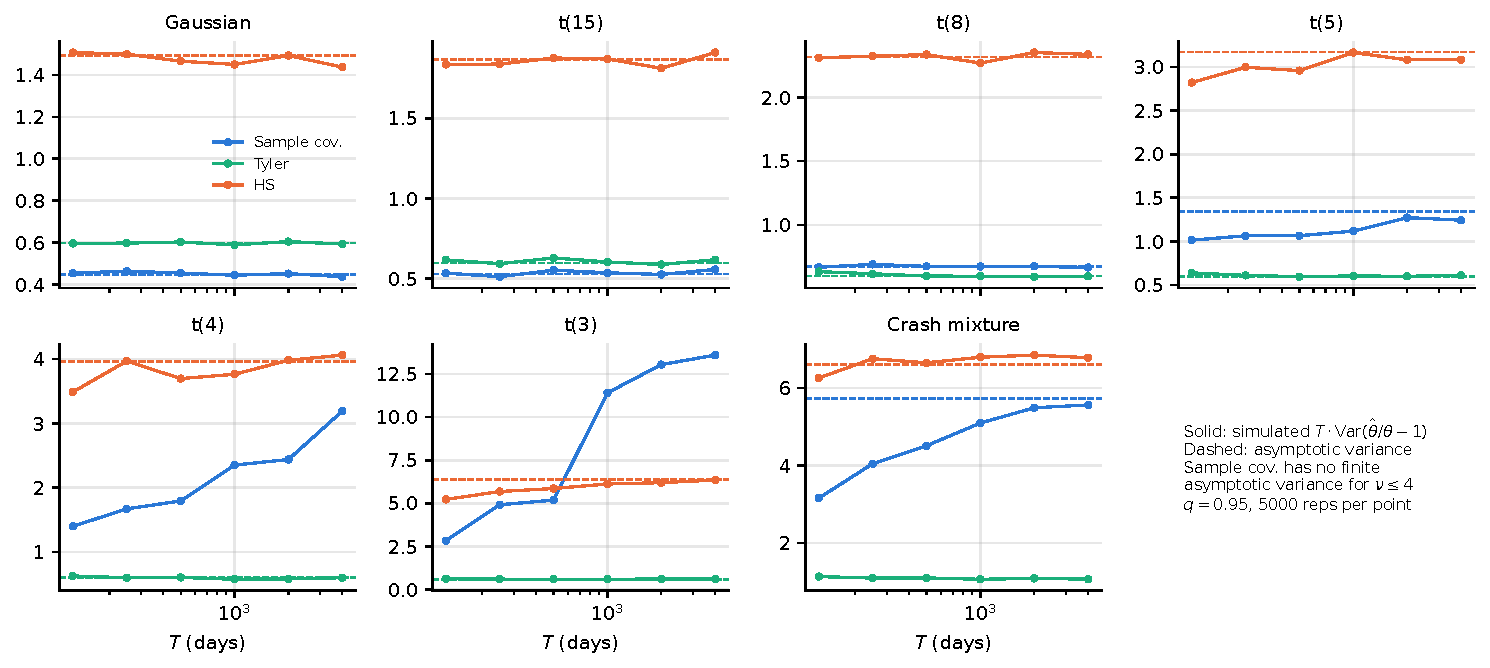
\includegraphics[width=\textwidth]{figures/est_tvar.pdf}
\caption{$T\cdot\Var(\hat\theta/\theta-1)$ by sample size, $q=0.95$. Dashed lines: asymptotic variances.}
\label{fig:tvar}
\end{figure}

\paragraph{Rates.}
Table~\ref{tab:rates} regresses the log interquartile range of each estimator's error on $\log T$. The
$\sqrt T$-consistent cases have slopes between $-0.47$ and $-0.52$, except the sample covariance at $t_5$
($-0.459$) and HS at $t_3$ ($-0.442$), where convergence is slow over this range of $T$. For the sample-covariance ratio the slope is $-0.332$ at $t_3$, against $-1/3$ from
Proposition~\ref{prop:stable}(a), and $-0.431$ at $t_4$, against about $-0.42$ for $\sqrt{\log T/T}$ over this
range. Variance slopes give $-0.56$ and $-0.75$ instead (relative to $-1$ for $\sqrt T$), which is what one
expects when the limit has infinite variance.

\begin{table}[H]
\centering\small
\caption{Slope of $\log\mathrm{IQR}(\hat\theta/\theta-1)$ on $\log T$, $T=125,\dots,4000$, $q=0.95$. $\sqrt T$
convergence corresponds to $-0.5$.}
\label{tab:rates}
\begin{tabular}{lrrrr}
\toprule
DGP & Predicted (sample cov.) & Sample cov. & Tyler & HS \\
\midrule
Gaussian & $-$0.500 & $-$0.504 & $-$0.494 & $-$0.503 \\
$t_{15}$ & $-$0.500 & $-$0.501 & $-$0.499 & $-$0.490 \\
$t_8$ & $-$0.500 & $-$0.505 & $-$0.507 & $-$0.490 \\
$t_5$ & $-$0.500 & $-$0.459 & $-$0.507 & $-$0.473 \\
$t_4$ & $-$0.424 & $-$0.431 & $-$0.514 & $-$0.477 \\
$t_3$ & $-$0.333 & $-$0.332 & $-$0.501 & $-$0.442 \\
\bottomrule
\end{tabular}
\end{table}

\paragraph{Confidence intervals.}
Table~\ref{tab:cov} reports the coverage of nominal 95\% intervals $\hat\theta(1\pm1.96\sqrt{\hat V/T})$ built
from Propositions~\ref{prop:clt}--\ref{prop:hs}, with 2{,}000 replications. Tyler's interval covers 94.2--95.7\%
in every elliptical cell, with a width that does not depend on $\nu$. The sample-covariance interval is accurate
for $\nu\ge8$ and under-covers in small samples with heavy tails (89.5\% at $t_3$, $T=250$). At $t_3$ its
coverage recovers to 94.1\% at $T=4000$, but this is not guaranteed: for $\alpha<2$ the Studentised statistic
behaves like a self-normalised sum, whose limit is not normal \citep{logan1973}; and the interval is 2.5 times
as wide as Tyler's. HS is accurate from $T=1000$.

\begin{table}[H]
\centering\small
\caption{Coverage (\%) of nominal 95\% intervals for the true ES ratio, $q=0.95$, 2{,}000 replications
(Monte Carlo s.e.\ about 0.5 points), by sample size $T$.}
\label{tab:cov}
\begin{tabular}{lrrrrrrrrr}
\toprule
 & \multicolumn{3}{c}{Sample covariance} & \multicolumn{3}{c}{Tyler} & \multicolumn{3}{c}{HS} \\
\cmidrule(lr){2-4}\cmidrule(lr){5-7}\cmidrule(lr){8-10}
DGP & 250 & 1000 & 4000 & 250 & 1000 & 4000 & 250 & 1000 & 4000 \\
\midrule
Gaussian & 94.4 & 95.5 & 94.5 & 94.8 & 95.2 & 94.8 & 93.2 & 95.2 & 95.0 \\
$t_8$ & 94.0 & 94.0 & 94.5 & 94.5 & 94.8 & 94.2 & 93.2 & 94.5 & 94.8 \\
$t_5$ & 92.5 & 94.0 & 93.5 & 94.5 & 95.5 & 95.1 & 92.6 & 94.3 & 94.2 \\
$t_4$ & 91.9 & 93.9 & 94.5 & 94.6 & 95.7 & 94.2 & 92.7 & 95.0 & 94.7 \\
$t_3$ & 89.5 & 92.8 & 94.1 & 94.2 & 94.5 & 95.0 & 92.2 & 95.1 & 94.2 \\
Crash mixture & 61.4 & 56.5 & 29.2 & 0.4 & 0.0 & 0.0 & 84.0 & 94.0 & 94.3 \\
\midrule
\multicolumn{10}{l}{\emph{Median width (\% of $\theta$), $T=4000$}} \\
Gaussian & \multicolumn{3}{c}{4.1} & \multicolumn{3}{c}{4.8} & \multicolumn{3}{c}{7.6} \\
$t_4$ & \multicolumn{3}{c}{7.6} & \multicolumn{3}{c}{4.8} & \multicolumn{3}{c}{12.1} \\
$t_3$ & \multicolumn{3}{c}{12.1} & \multicolumn{3}{c}{4.8} & \multicolumn{3}{c}{14.4} \\
Crash mixture & \multicolumn{3}{c}{12.3} & \multicolumn{3}{c}{4.9} & \multicolumn{3}{c}{15.8} \\
\bottomrule
\end{tabular}
\end{table}

\paragraph{When the structure fails.}
Under the crash mixture the sample-covariance and Tyler ratios converge to the wrong value. Write
$\beta=\theta_G/\theta-1$; ignoring $O(1/T)$ terms, $\mathrm{MSE}_G\approx\beta^2+V_G/T$ and
$\mathrm{MSE}_{HS}\approx V_{HS}/T$, so HS wins after $T^*\approx(V_{HS}-V_G)/\beta^2$. With $\beta$, $V_G$ and
$V_{HS}$ computed from influence functions on a $10^7$-day sample, $T^*$ is 110, 54 and 6 at $q=0.95,0.975,0.99$;
in the simulation HS first wins at the grid points 250, 125 and 125 (its own small-sample bias delays the
crossover at $q=0.95$). Figure~\ref{fig:crash} shows that the approximation tracks the simulated RMSE at $q=0.95$ and $0.975$; at $q=0.99$ only about 40 tail observations enter HS at $T=4000$, and its small-sample bias keeps its RMSE above $\sqrt{V_{HS}/T}$ over the whole grid. Tyler is
the worst of the three: its limit is 27\%, 45\% and 84\% above $\theta$, against 9\%, 25\% and 59\% for the
sample covariance. Tyler down-weights large observations, and the large joint crashes are exactly what
determines ES here. The intervals built on the two structural estimators cover the true ratio less and less
often as $T$ grows (Tyler 0\%); only the HS interval is valid.

\begin{figure}[H]
\centering
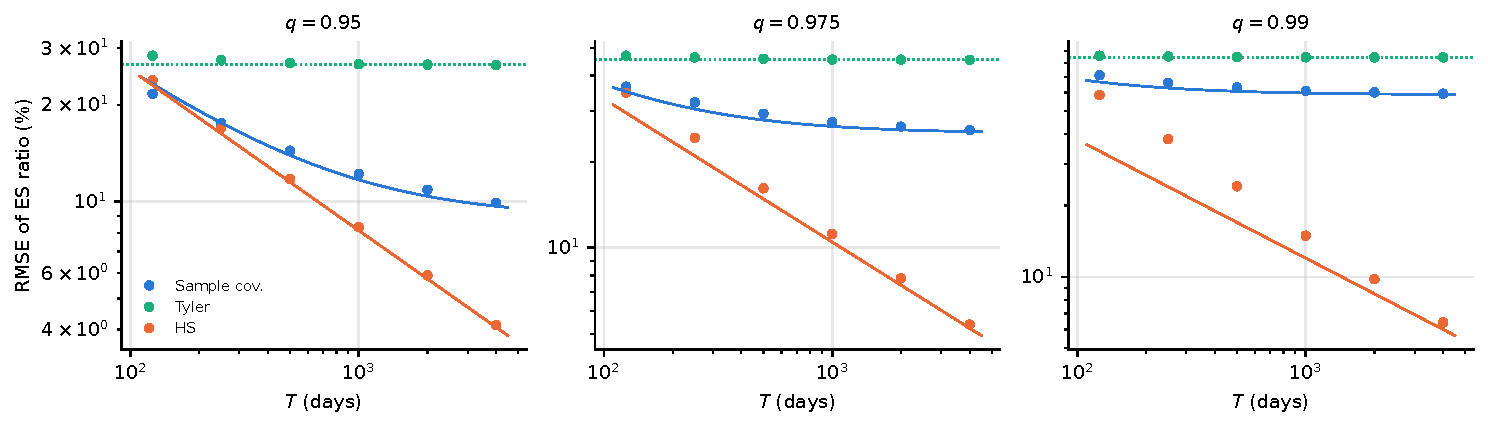
\includegraphics[width=\textwidth]{figures/est_crash.pdf}
\caption{Crash mixture: RMSE of the ES ratio. Points: simulation. Solid lines: $\sqrt{\beta^2+V_G/T}$ for the
sample covariance and $\sqrt{V_{HS}/T}$ for HS. Dotted line: Tyler's asymptotic bias.}
\label{fig:crash}
\end{figure}

% ---------------------------------------------------------------------------
\section{What is known, what is derived here, what is only simulated}\label{sec:contrib}

\begin{table}[H]
\centering\small
\begin{tabular}{p{0.47\textwidth}p{0.45\textwidth}}
\toprule
Result & Status \\
\midrule
ES $=-w^\top\mu+k_q\sigma_w$ under ellipticity; ES ratio $=\sigma_{w_1}/\sigma_{w_2}$ (Prop.~\ref{prop:es}) & Known \citep{mcneil2015}; proof included \\
Min ES $\Leftrightarrow$ min variance, ES parity $\Leftrightarrow$ volatility parity & Known \citep{tasche1999,mcneil2015} \\
Non-zero mean: ratio preserved iff equal Sharpe ratios (Prop.~\ref{prop:bound}(i)) & Derived here (elementary) \\
Consistency of the three estimators (Prop.~\ref{prop:cons}) & (a) proved; (b), (c) cited \\
$V_G=\frac14\Var(U_1^2-U_2^2)$, $(1+\kappa)(1-\rho^2)$ under ellipticity (Prop.~\ref{prop:clt}, Cor.~\ref{cor:vg}) & Derived here with the delta method \\
$V_{\mathrm{Ty}}=\frac{d+2}d(1-\rho^2)$ (Prop.~\ref{prop:tyler}) & From \citet{tyler1987} plus delta method; sample-mean centring only sketched \\
Efficiency crossover $\nu<d+4$ (Cor.~\ref{cor:eff}) & Derived here; confirmed by simulation \\
HS asymptotic normality (Prop.~\ref{prop:hs}) & Cited \citep{chen2008} \\
Rate $T^{-(1-2/\nu)}$ and $(\nu/2)$-stable limit for $2<\nu<4$ (Prop.~\ref{prop:stable}) & Derived here from standard tools; confirmed by IQR slopes \\
Crossover sample size $T^*$ under misspecification & Heuristic approximation; agrees with simulation \\
Tyler worse than the sample covariance under the crash mixture & Simulation finding for one DGP \\
\bottomrule
\end{tabular}
\end{table}

An earlier informal version of this project described the limit in Proposition~\ref{prop:stable} as a scale
mixture of normals. That would need a conditional Lindeberg condition, which fails because $W^2$ has tail index
$\alpha/2<1$; the stable limit replaces it, and the rate is unaffected.

% ---------------------------------------------------------------------------
\section{Limitations}

\begin{itemize}
\item \emph{Independence.} All theory and simulation assume i.i.d.\ returns. Volatility clustering changes both
the asymptotic variances and the validity of the intervals; the dynamic experiment in study~09 (GJR-GARCH) is
not covered by this theory.
\item \emph{One universe, two portfolios.} Results are for one covariance matrix with $d=6$ and one pair of
portfolios. The constant $\rho$ enters every asymptotic variance; the crossover $\nu<d+4$ moves with $d$.
\item \emph{One non-elliptical alternative.} The crash mixture is a single, deliberately strong departure. The
ranking of the sample covariance and Tyler under misspecification may differ for other departures.
\item \emph{Gaps in the proofs.} Tyler's asymptotics with an estimated centre (Proposition~\ref{prop:tyler}) are
only sketched; the necessary uniformity conditions are not verified, although the simulated variances agree
with the formula. We do not characterise the distributions for which the ratio identity holds at a single
level $q$.
\item \emph{Intervals under heavy tails.} For $2<\nu<4$ the sample-covariance interval has no asymptotic
guarantee; we report its simulated coverage only.
\item \emph{Decision relevance.} The link between ratio error and decision quality is simulation evidence from
study~09, not a theorem; a first-order expansion of decision regret in the estimation error is left for future
work.
\end{itemize}

% ---------------------------------------------------------------------------
\section{Conclusion}

When the decision depends on relative tail risk, a misspecified model can estimate it without bias, provided
the part of the structure it relies on is correct. In the elliptical family the choice is then between
estimators of shape, and it is governed by tail thickness: the sample covariance is best for light tails,
Tyler's estimator for $\nu<d+4$, and when fourth moments are missing the sample covariance loses its
$\sqrt T$ rate while Tyler keeps it. The same reasoning warns against relying on structure that is not there:
under a non-elliptical crash mixture with the correct covariance, the more robust the shape estimator, the
further it is from the ES ratio, and only the non-parametric estimator is consistent. A natural next step is to
test the elliptical structure itself before choosing an estimator, and to extend the asymptotic theory to
dependent data.

% ---------------------------------------------------------------------------
\appendix
\section{Proofs for Section~\ref{sec:pop}}\label{app:pop}

\begin{proof}[Proof of Proposition~\ref{prop:es}]
The characteristic function of $X-\mu$ is $\psi(t^\top\Sigma t)$, so that of $w^\top(X-\mu)$ is
$\psi(s^2\sigma_w^2)$. Take $w_0$ with $\sigma_{w_0}=1$ and set $Z=w_0^\top(X-\mu)$; its characteristic function
$\psi(s^2)$ is real and even, so $Z$ is symmetric and $-w^\top(X-\mu)\overset d=\sigma_wZ$ for every $w$. ES is
law-invariant, translation-equivariant and positively homogeneous, so
$\ES_q(L_w)=-w^\top\mu+\sigma_w\ES_q(Z)$. Let $f(u)=\mathrm{VaR}_u(Z)$, non-decreasing with $\int_0^1f=\E Z=0$.
The averages of $f$ over $(0,q)$ and $(q,1)$ bracket $f(q^-)\le f(q^+)$ and have weighted mean zero, so
$k_q=\ES_q(Z)\ge0$, with equality only if $f$ is a.e.\ constant, i.e.\ $Z\equiv0$, which non-degeneracy rules
out. The ratio statements follow.
\end{proof}

\begin{proof}[Proof of Proposition~\ref{prop:bound}]
(i) By Proposition~\ref{prop:es}, $\theta=(k_q\sigma_{w_1}-w_1^\top\mu)/(k_q\sigma_{w_2}-w_2^\top\mu)$; factor
out $k_q\sigma_{w_j}$. Equality with $\theta_G$ holds iff $1-SR_1/k_q=1-SR_2/k_q$. (ii) is the counterexample in
the text: $\ES_{0.95}(-X_1)=k^N_{0.95}=2.063$ and $\ES_{0.95}(-X_2)=1$.
\end{proof}

\section{Proofs for Section~\ref{sec:asy}}\label{app:asy}

\begin{lemma}\label{lem:g}
$g(cM)=g(M)$ for $c>0$, and $Dg(M)[H]=\tr(G_MH)$ with
\[
G_M=\frac{g(M)}2\left(\frac{w_1w_1^\top}{w_1^\top Mw_1}-\frac{w_2w_2^\top}{w_2^\top Mw_2}\right).
\]
Moreover $\tr(G_MM)=0$, and $\tr(G\Sigma G\Sigma)=\frac12\theta_G^2(1-\rho^2)$ for $G=G_\Sigma$.
\end{lemma}

\begin{proof}
Differentiate $\log g=\frac12\log(w_1^\top Mw_1)-\frac12\log(w_2^\top Mw_2)$. For the last identity, with
$A=w_1w_1^\top$, $B=w_2w_2^\top$: $\tr(A\Sigma A\Sigma)=\sigma_{w_1}^4$, $\tr(B\Sigma B\Sigma)=\sigma_{w_2}^4$ and
$\tr(A\Sigma B\Sigma)=\rho^2\sigma_{w_1}^2\sigma_{w_2}^2$.
\end{proof}

\begin{proof}[Proof of Proposition~\ref{prop:cons}]
(a) By the strong law, $S_T=\frac T{T-1}(\frac1T\sum_tX_tX_t^\top-\bar X\bar X^\top)\to\Sigma$ a.s., and $g$ is
continuous at $\Sigma$. (b) \citet{tyler1987} shows $\hat V_T\to c\Sigma$ a.s.; apply scale invariance.
(c) Both empirical ES converge a.s.\ \citep{acerbi2002} and the denominator's limit is positive.
\end{proof}

\begin{proof}[Proof of Proposition~\ref{prop:clt} and Corollary~\ref{cor:vg}]
With $Y=X-\mu$, $\sqrt T(S_T-\Sigma)=T^{-1/2}\sum_t(Y_tY_t^\top-\Sigma)+o_p(1)$, because $\sqrt T\,\bar Y\bar Y^\top=o_p(1)$.
The multivariate CLT gives $\sqrt T\vecop(S_T-\Sigma)\to N(0,\Gamma)$ with $\Gamma=\mathrm{Cov}(\vecop YY^\top)$. By
the delta method and Lemma~\ref{lem:g}, the asymptotic variance of $\sqrt T(\hat\theta_G-\theta_G)$ is
$\Var(\tr(GYY^\top))=\Var(\frac{\theta_G}2(U_1^2-U_2^2))$. Under ellipticity,
$\E[Y_iY_jY_kY_l]=(1+\kappa)(\sigma_{ij}\sigma_{kl}+\sigma_{ik}\sigma_{jl}+\sigma_{il}\sigma_{jk})$ \citep{muirhead1982},
so $\E U_j^4=3(1+\kappa)$, $\E U_1^2U_2^2=(1+\kappa)(1+2\rho^2)$ and
$\Var(U_1^2-U_2^2)=4(1+\kappa)(1-\rho^2)$. For unit-variance $t_\nu$, $\E U^4=3(\nu-2)/(\nu-4)$.
\end{proof}

\begin{proof}[Proof of Proposition~\ref{prop:tyler} (known centre) and Corollary~\ref{cor:eff}]
\citet{tyler1987} shows
$\sqrt T\vecop(\hat V_T-c\Sigma)\to N\big(0,\frac{d+2}d(I+K)(c\Sigma\otimes c\Sigma)+\sigma_2\vecop\Sigma\vecop\Sigma^\top\big)$,
with $K$ the commutation matrix, the factor $\frac{d+2}d$ free of the generator, and $\sigma_2$ depending only on
the normalisation. The second term is annihilated by $\tr(G\Sigma)=0$; the first gives
$\frac{d+2}d\cdot2\tr(G\Sigma G\Sigma)=\frac{d+2}d\theta^2(1-\rho^2)$. For the corollary, multiply
$(d+2)(\nu-4)<d(\nu-2)$ out: it is equivalent to $\nu<d+4$.
\end{proof}

\paragraph{Sketch for the estimated centre.}
$\hat V_T$ solves $\frac1T\sum_t\psi(X_t-m,V)=0$ with
\[
\psi(y,V)=\frac{d\,yy^\top}{y^\top V^{-1}y}-V .
\]
The $y$-part
is even and homogeneous of degree zero, so its derivative in $y$ is odd and homogeneous of degree $-1$; under a
symmetric distribution with $\E\|Y\|^{-1}<\infty$ (true for $d\ge2$) its expectation is zero, and a
$\sqrt T$-consistent centre has no first-order effect. A full proof needs stochastic equicontinuity in $m$,
which we do not verify. Simulated $T\cdot\Var$ agrees with $V_{\mathrm{Ty}}$ (Table~\ref{tab:three}).

\begin{proof}[Proof of Proposition~\ref{prop:stable}]
By scale invariance $\hat\theta_G=g(M_T-\bar Y\bar Y^\top)$ with $M_T=\frac1T\sum_tW_tZ_tZ_t^\top$, and
$\bar Y\bar Y^\top=O_p(T^{-1})$. Write $M_T-\Sigma=\frac1T\sum_t[W_tD_t+(W_t-\E W)\Sigma_0]$ with
$D_t=Z_tZ_t^\top-\Sigma_0$ and $\Sigma=\E W\,\Sigma_0$. Linearising and using $\tr(G\Sigma_0)=0$,
\[
\hat\theta_G-\theta=\frac1T\sum_tW_t\eta_t+O_p(\|M_T-\Sigma\|^2)+O_p(T^{-1}),\qquad\eta_t=\tr(GD_t),
\]
where $\eta_t$ is independent of $W_t$, has mean zero and all moments, and is non-degenerate when $|\rho|<1$. By
Breiman's lemma, $P(W\eta>x)\sim\E[\eta_+^\alpha]P(W>x)$ and $P(W\eta<-x)\sim\E[\eta_-^\alpha]P(W>x)$, so
$W_t\eta_t$ is regularly varying with index $\alpha$ in both tails. (a) For $1<\alpha<2$ the generalised central
limit theorem \citep[Ch.~XVII]{feller1971} gives $a_T^{-1}\sum_tW_t\eta_t\to\mathcal S_\alpha$ with
$a_T\propto T^{1/\alpha}$ and skewness $(\E\eta_+^\alpha-\E\eta_-^\alpha)/(\E\eta_+^\alpha+\E\eta_-^\alpha)$. The same
argument entrywise gives $\|M_T-\Sigma\|=O_p(a_T/T)$, so the remainders are $o_p(a_T/T)$. (b) For $\alpha=2$ the
truncated second moment of $W\eta$ grows like $\log x$, so $W\eta$ is in the domain of attraction of the normal
law with $a_T\asymp\sqrt{T\log T}$.
\end{proof}

% ---------------------------------------------------------------------------
\bibliographystyle{plainnat}
\begin{thebibliography}{99}

\bibitem[Acerbi and Tasche(2002)]{acerbi2002}
Acerbi, C. and Tasche, D. (2002). On the coherence of expected shortfall. \emph{Journal of Banking \& Finance},
26(7), 1487--1503.

\bibitem[Chen(2008)]{chen2008}
Chen, S. X. (2008). Nonparametric estimation of expected shortfall. \emph{Journal of Financial Econometrics},
6(1), 87--107.

\bibitem[Feller(1971)]{feller1971}
Feller, W. (1971). \emph{An Introduction to Probability Theory and Its Applications}, Vol.~II, 2nd ed. Wiley.

\bibitem[Logan et~al.(1973)]{logan1973}
Logan, B. F., Mallows, C. L., Rice, S. O. and Shepp, L. A. (1973). Limit distributions of self-normalized sums.
\emph{Annals of Probability}, 1(5), 788--809.

\bibitem[McNeil et~al.(2015)]{mcneil2015}
McNeil, A. J., Frey, R. and Embrechts, P. (2015). \emph{Quantitative Risk Management: Concepts, Techniques and
Tools}, revised ed. Princeton University Press.

\bibitem[Muirhead(1982)]{muirhead1982}
Muirhead, R. J. (1982). \emph{Aspects of Multivariate Statistical Theory}. Wiley.

\bibitem[Tasche(1999)]{tasche1999}
Tasche, D. (1999). Risk contributions and performance measurement. Working paper, Technische Universit\"at
M\"unchen.

\bibitem[Tyler(1987)]{tyler1987}
Tyler, D. E. (1987). A distribution-free M-estimator of multivariate scatter. \emph{Annals of Statistics},
15(1), 234--251.

\end{thebibliography}

\end{document}
